\documentclass[aspectratio=169,10pt]{beamer}

\usepackage[utf8]{inputenc}
\usepackage[T1]{fontenc}
\usepackage[spanish,es-nodecimaldot,es-noshorthands,es-tabla]{babel}
\usepackage{booktabs}
\usepackage{multirow}
\usepackage{amsmath,amssymb}
\usepackage{tikz}
\usetikzlibrary{positioning,arrows.meta,shapes.geometric}

% ---- tema Madrid en azul ----
\usetheme{Madrid}
\definecolor{azul}{RGB}{31,78,140}
\definecolor{rojo}{RGB}{192,80,77}
\usecolortheme[named=azul]{structure}
\setbeamertemplate{navigation symbols}{}
\setbeamertemplate{itemize item}{\color{azul}$\blacktriangleright$}
\setbeamertemplate{itemize subitem}{\color{azul}$\triangleright$}
\setbeamercolor{block title}{bg=azul,fg=white}
\setbeamercolor{block body}{bg=azul!8}

\graphicspath{{figuras/}{../paper/figuras/}}
\newcommand{\x}{$\times$}
% fuente al pie de cada diapositiva
\newcommand{\fuente}[1]{\vfill{\scriptsize\color{gray}Fuente: #1}}
% frase de cierre de la diapositiva
\newcommand{\nota}[1]{\begin{center}\colorbox{azul!10}{\parbox{0.94\textwidth}{\centering\small #1}}\end{center}}

\title[Búsqueda de ParlayANN en GPU]{Búsqueda de ParlayANN en GPU}
\subtitle{Comparación de los cuatro algoritmos en CPU y GPU sobre los mismos grafos}
\author[Iman, Tejeda y Nadeau]{Samuel Iman Quispe \and Juan Victor Tejeda \and Jean Marc Nadeau Huamani}
\institute[Ciencia de la Computación]{Ciencia de la Computación -- UCSP\\ Computación Paralela}
\date{Noviembre de 2026}

\begin{document}

\begin{frame}
  \titlepage
\end{frame}

% ============================================================================
\begin{frame}{01 \quad Qué propone ParlayANN y qué hicimos nosotros}
  \begin{columns}[T]
    \begin{column}{0.47\textwidth}
      \textbf{Propuesta del paper}
      \begin{itemize}
        \item Construir índices de búsqueda aproximada de vecinos cercanos (ANNS) con grafos.
        \item Paralelizar cuatro algoritmos sin usar locks.
        \item Que el resultado sea el mismo en cada corrida (determinista).
        \item Todo en CPU multinúcleo.
      \end{itemize}
    \end{column}
    \begin{column}{0.47\textwidth}
      \textbf{Lo que hicimos}
      \begin{itemize}
        \item Tomar los mismos grafos que construye ParlayANN.
        \item Programar la búsqueda de los cuatro algoritmos en CUDA.
        \item Comprobar que la GPU devuelve los mismos vecinos que la CPU.
        \item Medir CPU contra GPU en dos laptops distintas.
      \end{itemize}
    \end{column}
  \end{columns}
  \vspace{6pt}
  \nota{Si la GPU devuelve exactamente lo mismo que la CPU, la diferencia de tiempo se
  debe solo al hardware y no a un algoritmo distinto.}
  \fuente{Manohar et al., PPoPP 2024; repositorio ParlayANN-GPU-Busqueda.}
\end{frame}

% ============================================================================
\begin{frame}{02 \quad Cómo se busca en un grafo}
  \begin{columns}[c]
    \begin{column}{0.5\textwidth}
      \begin{itemize}
        \item Se empieza en el punto 0 con una frontera de $L_s$ candidatos.
        \item Se toma el más cercano que todavía no se visitó.
        \item Se leen sus vecinos y se descartan los que ya se vieron.
        \item Se calculan sus distancias y se mezclan con la frontera.
        \item Se recorta a $L_s$ y se repite hasta visitar toda la frontera.
      \end{itemize}
    \end{column}
    \begin{column}{0.47\textwidth}
      \centering
      \begin{tikzpicture}[
          nodo/.style={circle,draw=azul,fill=azul!10,minimum size=7mm,inner sep=0pt,font=\small},
          vis/.style={circle,draw=azul,fill=azul,text=white,minimum size=7mm,inner sep=0pt,font=\small},
          q/.style={star,star points=5,draw=rojo,fill=rojo!60,minimum size=6mm,inner sep=0pt}]
        \node[vis] (a) at (0,0) {0};
        \node[vis] (b) at (1.5,0.9) {};
        \node[nodo] (c) at (1.4,-0.9) {};
        \node[vis] (d) at (3,0.4) {};
        \node[nodo] (e) at (3.1,1.7) {};
        \node[nodo] (f) at (4.4,-0.4) {};
        \node[nodo] (g) at (4.6,1.0) {};
        \node[q] (q) at (5.3,0.3) {};
        \draw[-{Latex},thick,azul] (a) -- (b);
        \draw[-{Latex},thick,azul] (b) -- (d);
        \draw[-{Latex},thick,azul] (d) -- (g);
        \draw[gray] (a) -- (c) (b) -- (e) (c) -- (d) (d) -- (f) (f) -- (g) (e) -- (g);
        \node[font=\scriptsize,rojo] at (5.3,-0.25) {consulta};
        \node[font=\scriptsize,azul] at (1.5,-1.6) {en azul: nodos visitados};
      \end{tikzpicture}
    \end{column}
  \end{columns}
  \vspace{6pt}
  \nota{$L_s$ controla el balance: con un $L_s$ más grande se gana recall pero se atienden
  menos consultas por segundo.}
  \fuente{Paper, Sección 3; \texttt{beamSearch.h} del artefacto.}
\end{frame}

% ============================================================================
\begin{frame}{03 \quad Los cuatro algoritmos y sus grafos}
  \centering
  \begin{tabular}{llcc}
    \toprule
    Algoritmo & Cómo construye el grafo & Grado máx. & Grado prom. \\
    \midrule
    DiskANN     & Inserción por lotes y poda (grafo Vamana)     & 64  & 57.4 \\
    HCNNG       & Unión de árboles de expansión mínima           & 150 & 99.8 \\
    PyNNDescent & Árboles y refinamiento con vecinos de vecinos  & 60  & 41.4 \\
    HNSW        & Grafos en varios niveles                       & 64  & --- \\
    \bottomrule
  \end{tabular}
  \vspace{8pt}
  \begin{itemize}
    \item Dataset MSSPACEV-1M: 1\,000\,000 de vectores de 100 dimensiones, 29\,316 consultas, $k = 10$.
    \item Los grafos los construye ParlayANN en CPU y la GPU lee esos mismos archivos.
    \item HCNNG tiene 26.9 millones de aristas repetidas y PyNNDescent 5\,637; también
          hay que respetarlas.
  \end{itemize}
  \fuente{Grafos generados con ParlayANN (commit 45587ba); conteos propios.}
\end{frame}

% ============================================================================
\begin{frame}{04 \quad La búsqueda en GPU: un warp por consulta}
  \begin{columns}[c]
    \begin{column}{0.48\textwidth}
      \begin{itemize}
        \item Cada consulta la resuelve un warp de 32 hilos.
        \item Cada warp toma siempre las mismas consultas, así que no usamos atómicos y el
              resultado no cambia entre corridas.
        \item La frontera y los candidatos van en memoria compartida.
        \item Rellenamos los vectores de 100 a 128 bytes para leerlos de una vez.
        \item La distancia se calcula con \texttt{\_\_dp4a} usando solo enteros, así sale
              el mismo número que en la CPU.
      \end{itemize}
    \end{column}
    \begin{column}{0.5\textwidth}
      \centering
      \begin{tikzpicture}[font=\scriptsize,
          hilo/.style={draw=azul,fill=azul!15,minimum width=3.4mm,minimum height=5mm,inner sep=0pt},
          vec/.style={draw=azul,fill=azul,text=white,minimum width=1.25cm,minimum height=5mm}]
        \node[font=\small,azul] at (2.9,2.0) {Warp de 32 hilos = 4 grupos de 8};
        \foreach \g in {0,...,3} {
          \foreach \h in {0,...,7} {
            \node[hilo] at ({\g*1.5+\h*0.17},1.3) {};
          }
          \node[font=\tiny] at ({\g*1.5+0.6},0.85) {grupo \g};
          \draw[-{Latex},azul] ({\g*1.5+0.6},0.65) -- ({\g*1.5+0.6},0.15);
          \node[vec] at ({\g*1.5+0.6},-0.15) {vector};
        }
        \node[align=center] at (2.9,-1.0) {cada hilo lee 16 bytes, entre los 8\\
          leen el vector de 128 bytes};
        \node[align=center,azul] at (2.9,-1.7) {cada hilo lleva 4 distancias:
          16 vectores pedidos a la vez};
      \end{tikzpicture}
    \end{column}
  \end{columns}
  \fuente{\texttt{cuda/busqueda.cu}, \texttt{cuda/distancia.cuh}.}
\end{frame}

% ============================================================================
\begin{frame}{05 \quad Para que salga lo mismo que en la CPU}
  \begin{columns}[T]
    \begin{column}{0.47\textwidth}
      \textbf{Detalles que copiamos de ParlayANN}
      \begin{itemize}
        \item Inicio en el punto 0, $k = 10$ y corte en $1.35 \cdot d_k$.
        \item Filtro de ``ya visto'' con pérdidas: un vecino puede pisar la casilla de otro.
        \item Aristas repetidas: la frontera se maneja como multiconjunto.
        \item En HNSW los candidatos se ordenan solo por distancia y los vecinos se
              aceptan en orden.
      \end{itemize}
    \end{column}
    \begin{column}{0.47\textwidth}
      \textbf{Cómo lo resolvimos en paralelo}
      \begin{itemize}
        \item La CPU revisa el filtro vecino por vecino; en la GPU los 32 hilos leen todas
              las casillas de una vez.
        \item Con \texttt{\_\_match\_any\_sync} cada hilo sabe qué había en su casilla
              justo antes de él.
        \item En HNSW solo la decisión de quién entra va en orden; leer, filtrar y calcular
              distancias va en paralelo.
      \end{itemize}
    \end{column}
  \end{columns}
  \vspace{4pt}
  \nota{Copiar estos detalles fue necesario: sin ellos el recall ya no coincidía con el de
  la CPU.}
  \fuente{\texttt{beamSearch.h} y \texttt{HNSW.hpp} del artefacto; \texttt{cuda/busqueda\_hnsw.cu}.}
\end{frame}

% ============================================================================
\begin{frame}{06 \quad Optimizaciones del kernel}
  \begin{columns}[c]
    \begin{column}{0.62\textwidth}
      \centering
      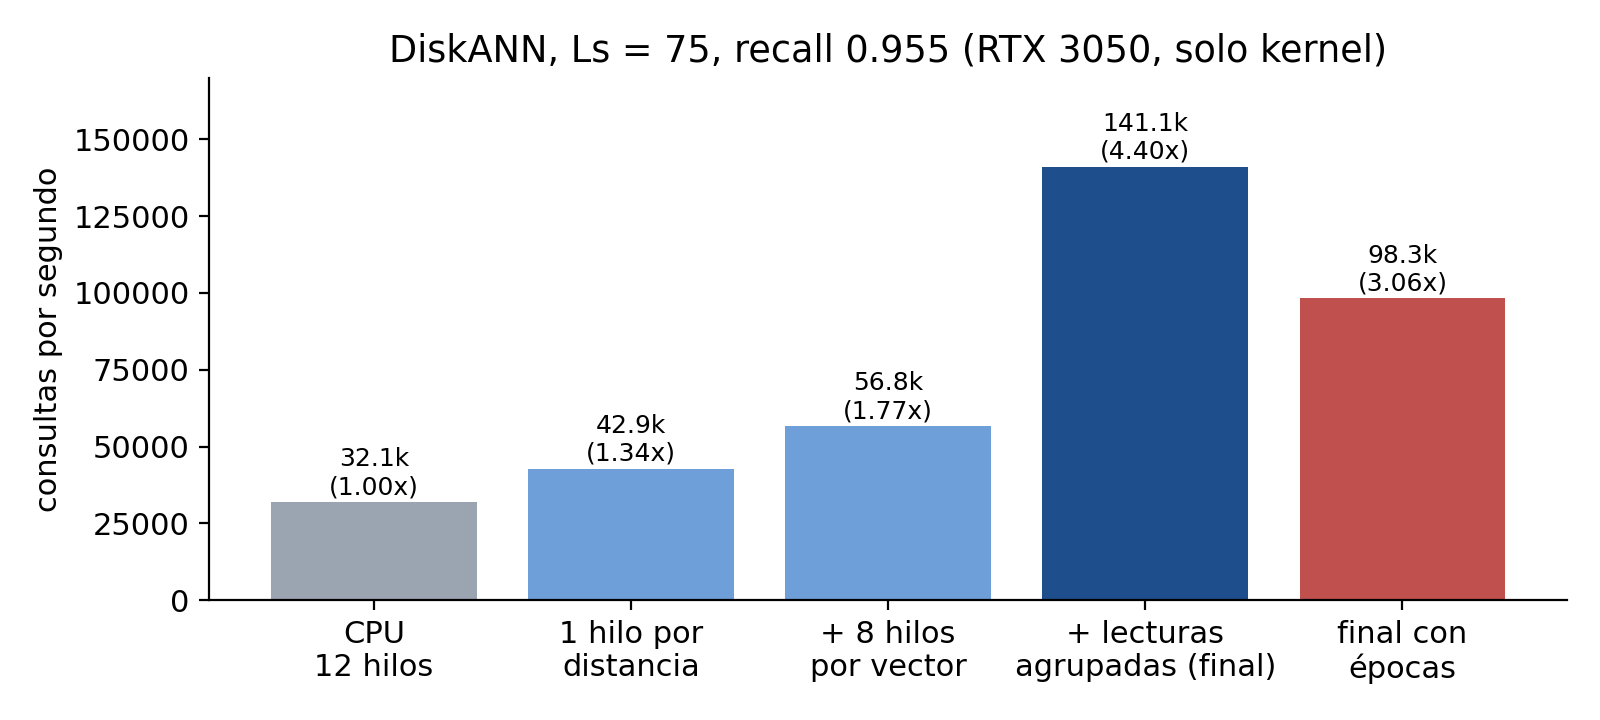
\includegraphics[width=\textwidth]{optimizaciones.png}
    \end{column}
    \begin{column}{0.36\textwidth}
      \begin{itemize}
        \item Primera versión: un hilo por distancia, apenas 1.34\x{} sobre la CPU.
        \item Leer cada vector con 8 hilos y pedir la fila de vecinos de una vez la llevó a
              4.40\x.
        \item Probamos no limpiar el filtro usando ``épocas'': salió 30\,\% más lento, así
              que lo descartamos.
      \end{itemize}
    \end{column}
  \end{columns}
  \fuente{Mediciones propias en la RTX 3050, DiskANN con $L_s = 75$, una corrida.}
\end{frame}

% ============================================================================
\begin{frame}{07 \quad Hardware y forma de medir}
  \begin{columns}[T]
    \begin{column}{0.52\textwidth}
      \centering
      \small\setlength{\tabcolsep}{4pt}
      \begin{tabular}{lll}
        \toprule
        Recurso & Máquina A & Máquina B \\
        \midrule
        CPU      & i5-12450HX      & i7-13700HX \\
        Hilos    & 12              & 24 \\
        RAM      & 24 GB DDR5      & 16 GB DDR5 \\
        GPU      & RTX 3050 Laptop & RTX 5050 Laptop \\
        Arquitectura & Ampere      & Blackwell \\
        VRAM     & 6 GB            & 8 GB \\
        \bottomrule
      \end{tabular}
    \end{column}
    \begin{column}{0.45\textwidth}
      \begin{itemize}
        \item 4 algoritmos \x{} 18 configuraciones = 72 mediciones por máquina.
        \item Una corrida de calentamiento y nos quedamos con la mejor de 5.
        \item En la GPU medimos de punta a punta: copiar consultas, kernel y traer
              resultados.
        \item CPU con todos sus hilos y laptops en modo de máximo rendimiento.
      \end{itemize}
    \end{column}
  \end{columns}
  \vspace{6pt}
  \nota{Las dos máquinas no son equivalentes: comparamos CPU y GPU dentro de cada una, y
  después comparamos las dos generaciones.}
  \fuente{\texttt{comparacion1\_equipo*.txt}; \texttt{hardware.txt} de cada corrida de CPU.}
\end{frame}

% ============================================================================
\begin{frame}{08 \quad ¿La GPU devuelve lo mismo que la CPU?}
  \centering
  \begin{tabular}{lccccc}
    \toprule
     & Recall & \multicolumn{2}{c}{Mismos 10 vecinos} & Mismas & Determinista \\
    Algoritmo & idéntico & A & B & distancias & (A y B) \\
    \midrule
    DiskANN     & 18/18 & 100 \% & 100 \% & 100 \% & 18/18 \\
    HCNNG       & 18/18 & 100 \% & 100 \% & 100 \% & 18/18 \\
    PyNNDescent & 18/18 & 100 \% & 100 \% & 100 \% & 18/18 \\
    HNSW        & 18/18 & 99.42 \% & 99.44 \% & 100 \% & 18/18 \\
    \bottomrule
  \end{tabular}
  \vspace{10pt}
  \begin{itemize}
    \item Las 72 configuraciones dan el mismo recall en las dos máquinas.
    \item En HNSW, los vecinos que cambian están a la misma distancia: son empates que la
          CPU resuelve de otra forma.
  \end{itemize}
  \fuente{\texttt{validacion.csv}, comparación consulta por consulta con los HDF5 de la CPU.}
\end{frame}

% ============================================================================
\begin{frame}{09 \quad Speedup con recall $\geq$ 0.95}
  \begin{columns}[c]
    \begin{column}{0.6\textwidth}
      \centering
      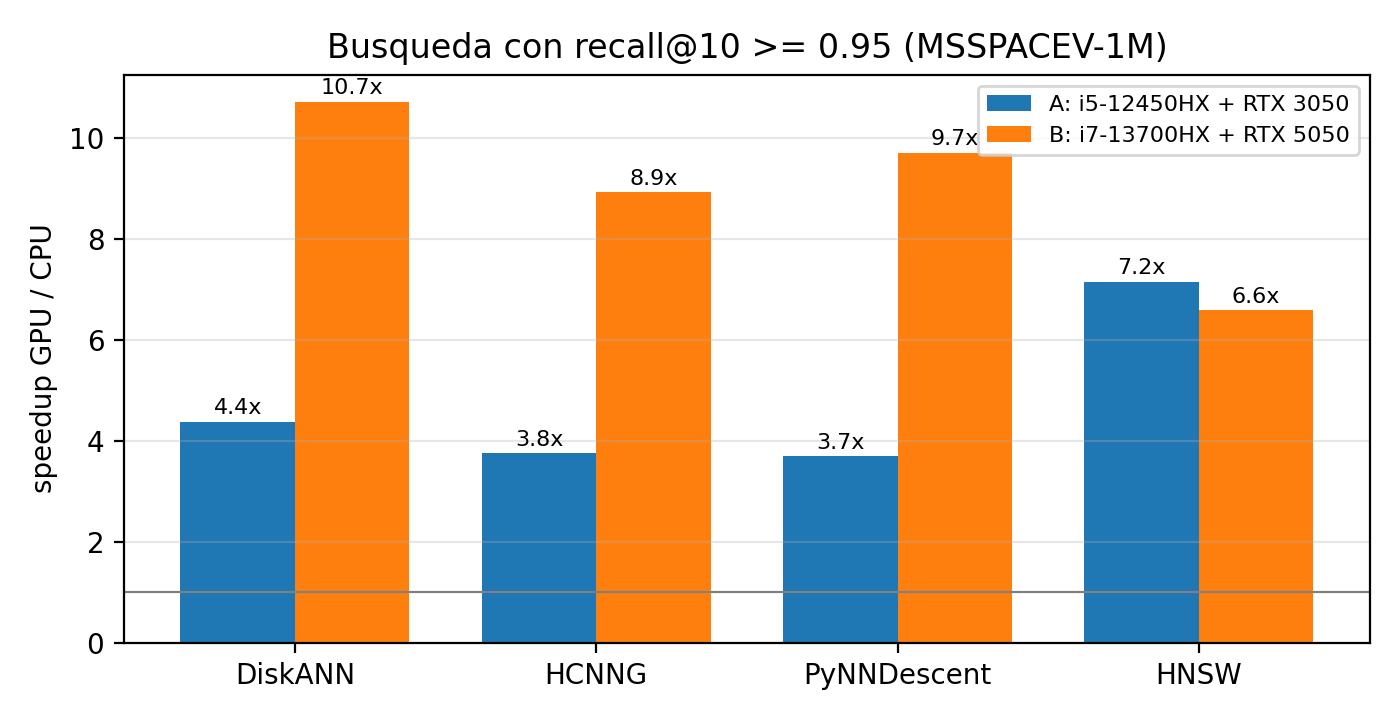
\includegraphics[width=\textwidth]{speedup_maquinas.png}
    \end{column}
    \begin{column}{0.38\textwidth}
      \begin{itemize}
        \item Máquina A: entre 3.7\x{} y 7.2\x.
        \item Máquina B: entre 6.6\x{} y 10.7\x.
        \item La GPU fue más rápida en las 72 configuraciones.
        \item Copiar los datos entre CPU y GPU cuesta menos del 2 \% con este recall.
      \end{itemize}
    \end{column}
  \end{columns}
  \fuente{\texttt{paper/comparacion\_maquinas.md}.}
\end{frame}

% ============================================================================
\begin{frame}{10 \quad ¿Qué rendimiento obtuvimos a alto recall?}
  \centering
  {\small Mejor QPS entre las configuraciones con recall@10 $\geq$ 0.95.}\\[6pt]
  {\small\setlength{\tabcolsep}{4.5pt}
  \begin{tabular}{lrrrrrrrr}
    \toprule
     & \multicolumn{3}{c}{Máquina A (i5 + RTX 3050)} & \multicolumn{3}{c}{Máquina B (i7 + RTX 5050)}
     & \multicolumn{2}{c}{Mejora B/A} \\
    \cmidrule(lr){2-4}\cmidrule(lr){5-7}\cmidrule(lr){8-9}
    Algoritmo & CPU & GPU & Speedup & CPU & GPU & Speedup & CPU & GPU \\
    \midrule
    DiskANN     & 32\,079 & 140\,531 & 4.4\x & 52\,325 & 561\,297 & 10.7\x & 1.63\x & 3.99\x \\
    HCNNG       & 19\,936 & 74\,808  & 3.8\x & 28\,150 & 251\,385 & 8.9\x  & 1.41\x & 3.36\x \\
    PyNNDescent & 44\,258 & 163\,524 & 3.7\x & 62\,352 & 605\,957 & 9.7\x  & 1.41\x & 3.71\x \\
    HNSW        & 7\,350  & 52\,635  & 7.2\x & 16\,530 & 108\,921 & 6.6\x  & 2.25\x & 2.07\x \\
    \bottomrule
  \end{tabular}}
  \vspace{8pt}
  \nota{En DiskANN, HCNNG y PyNNDescent la CPU mejoró entre 1.4\x{} y 1.6\x{} de una
  generación a otra (con el doble de hilos) y la GPU entre 3.4\x{} y 4.0\x. HNSW es la
  excepción: 2.25\x{} y 2.07\x.}
  \fuente{\texttt{configuraciones.csv} de cada máquina; cada celda es el mejor punto del barrido que cumple el recall.}
\end{frame}

% ============================================================================
\begin{frame}{11 \quad Curvas recall -- QPS}
  \centering
  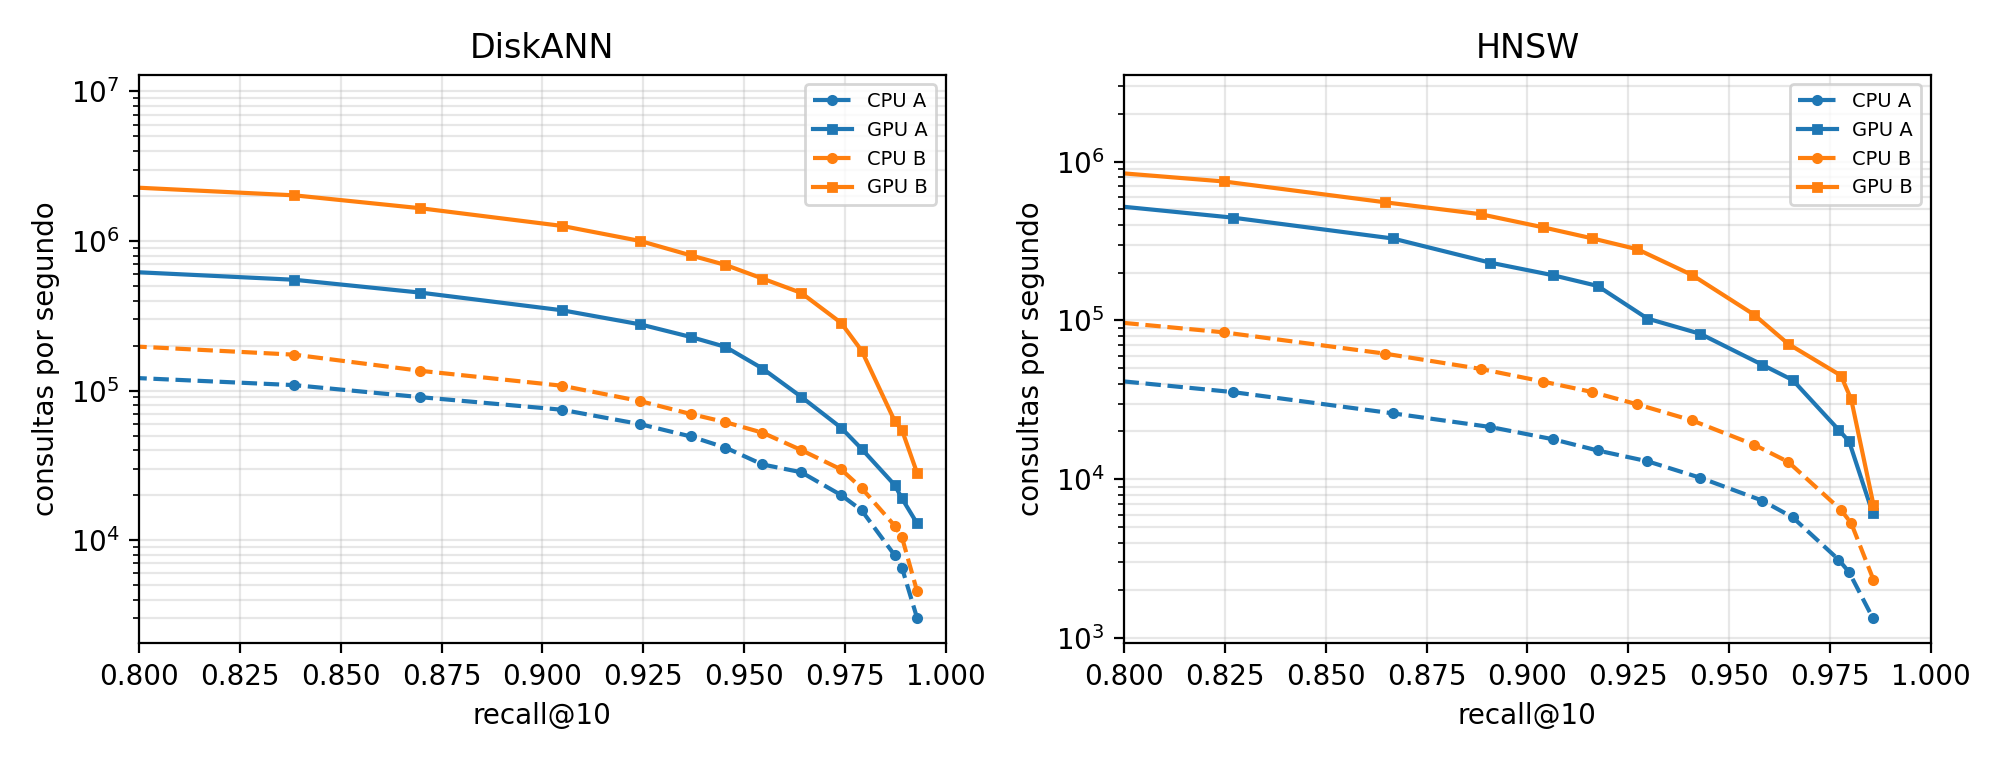
\includegraphics[width=0.9\textwidth]{recall_qps_maquinas.png}\\[2pt]
  {\small Punteado: CPU. Continuo: GPU de punta a punta. El eje vertical está en escala logarítmica.}
  \fuente{Mismas 18 configuraciones de \texttt{artifact\_eval.yaml} en las dos máquinas.}
\end{frame}

% ============================================================================
\begin{frame}{12 \quad ¿Qué limita al kernel?}
  \begin{columns}[c]
    \begin{column}{0.5\textwidth}
      \centering
      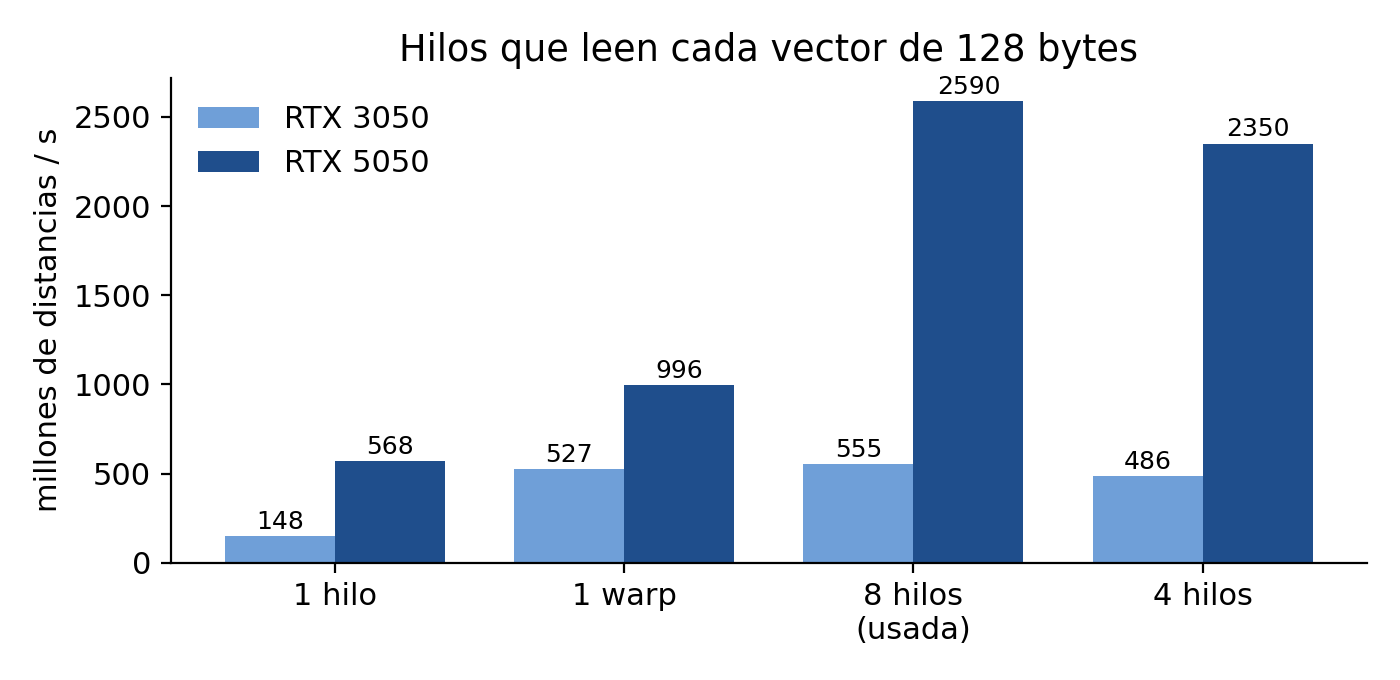
\includegraphics[width=\textwidth]{microbenchmark.png}
    \end{column}
    \begin{column}{0.5\textwidth}
      \centering
      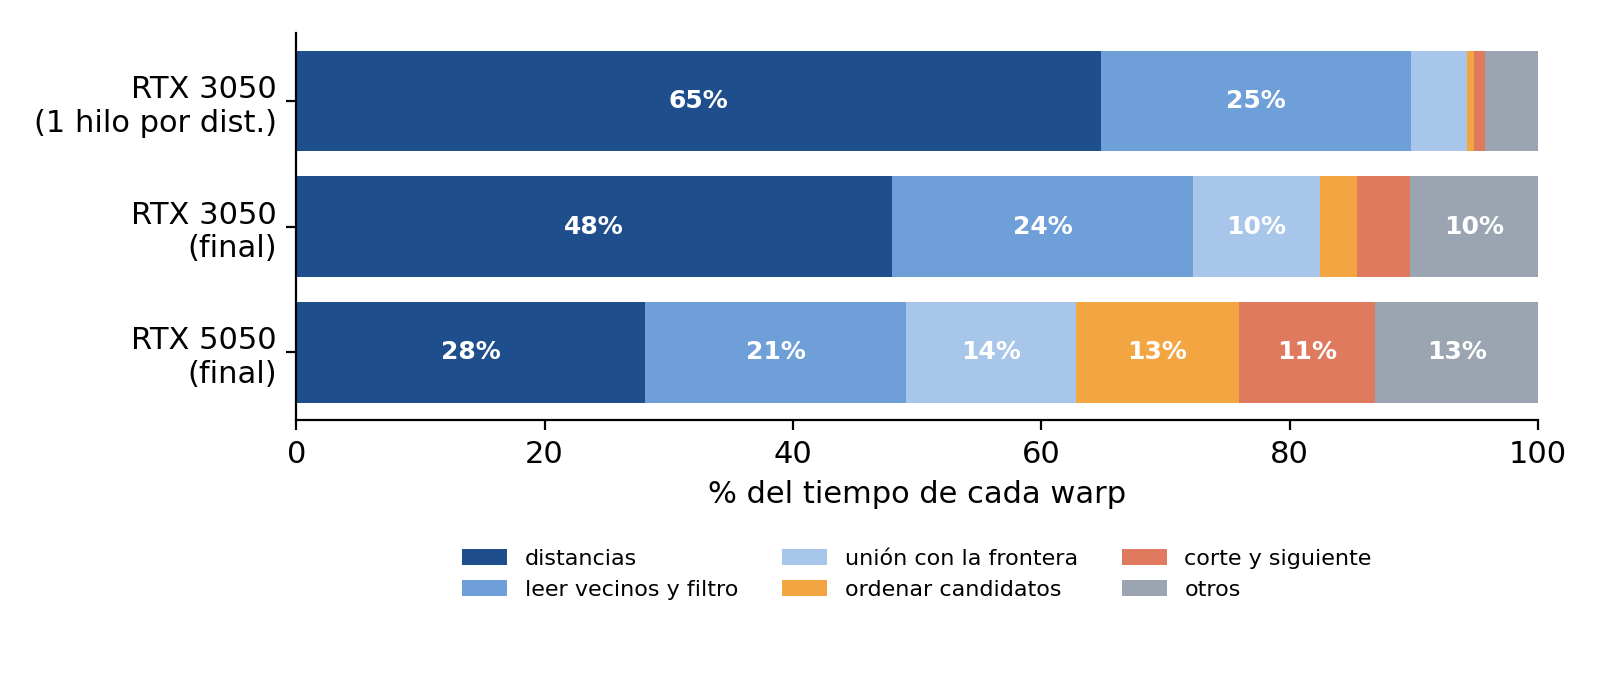
\includegraphics[width=\textwidth]{perfil.png}
    \end{column}
  \end{columns}
  \begin{itemize}
    \item En la RTX 3050 el kernel calcula 499 millones de distancias por segundo, el 90 \%
          de lo que da el microbenchmark: lo frena el acceso a memoria.
    \item En la RTX 5050 las distancias bajan al 28 \% del tiempo y empiezan a pesar ordenar,
          la unión y el corte.
  \end{itemize}
  \fuente{\texttt{micro\_distancias.txt} y \texttt{perfil\_diskann\_75.txt} (DiskANN, $L_s = 75$).}
\end{frame}

% ============================================================================
\begin{frame}{13 \quad Conclusiones de la comparación}
  \begin{columns}[T]
    \begin{column}{0.47\textwidth}
      \textbf{Conclusiones comprobadas}
      \begin{itemize}
        \item La GPU devuelve lo mismo que la CPU en las 72 configuraciones.
        \item Con recall $\geq$ 0.95 es entre 3.7\x{} y 10.7\x{} más rápida.
        \item En DiskANN, HCNNG y PyNNDescent la GPU mejoró más que la CPU entre
              generaciones.
        \item HNSW escala menos porque una parte de su búsqueda es secuencial.
      \end{itemize}
    \end{column}
    \begin{column}{0.47\textwidth}
      \textbf{Limitaciones del experimento}
      \begin{itemize}
        \item Un solo dataset de un millón de puntos.
        \item Son laptops: influyen la temperatura y el modo de energía.
        \item HCNNG, PyNNDescent y HNSW quedaron con grafos algo distintos en cada máquina.
        \item La construcción de los grafos sigue en la CPU.
      \end{itemize}
    \end{column}
  \end{columns}
  \vspace{6pt}
  \nota{Balance: búsqueda en GPU equivalente a la de ParlayANN, más rápida en las dos
  máquinas y verificada consulta por consulta.}
\end{frame}

% ============================================================================
\begin{frame}{14 \quad Trabajo futuro}
  \begin{enumerate}
    \item \textbf{Construcción de grafos en GPU}\\
          Empezar por DiskANN y HNSW, que insertan por lotes y comparten casi todo el código.
          Medir tiempo, calidad del grafo y determinismo.
    \item \textbf{Datasets más grandes}\\
          Probar con 10 millones de puntos o más, mientras quepan en la memoria de la GPU.
    \item \textbf{HNSW}\\
          Reducir la parte secuencial que limita su speedup con $L_s$ grandes.
  \end{enumerate}
  \fuente{Propuestas propias a partir de las limitaciones encontradas.}
\end{frame}

% ============================================================================
\begin{frame}{15 \quad Referencias y materiales}
  \footnotesize
  \begin{enumerate}
    \item M. D. Manohar, Z. Shen, G. E. Blelloch, L. Dhulipala, Y. Gu, H. V. Simhadri y Y. Sun.
          \textit{ParlayANN: Scalable and Deterministic Parallel Graph-Based Approximate
          Nearest Neighbor Search Algorithms}. PPoPP 2024.
    \item S. J. Subramanya et al. \textit{DiskANN}. NeurIPS 2019. \quad
          Y. A. Malkov y D. A. Yashunin. \textit{HNSW}. IEEE TPAMI 2020.
    \item H. Ootomo et al. \textit{CAGRA: Highly Parallel Graph Construction and ANN Search
          for GPUs}. ICDE 2024.
    \item H. V. Simhadri et al. \textit{Results of the NeurIPS'21 Challenge on Billion-Scale
          ANN Search}. PMLR 176, 2022.
    \item Código y resultados: \url{https://github.com/Jean-Marc-NH/ParlayANN-GPU-Busqueda}
  \end{enumerate}
  \vfill
  \centering
  {\Large\color{azul} Gracias}
  \vfill
\end{frame}

\end{document}
